% !TEX root =  root.tex


\section{METHODS}
\label{sec:methods}
\subsection*{Verification}
To verify if a matrix $A$ was inverted correctly one has to check if equation (\ref{eq:inverse}) holds. So our implementation also requires functions to multiply two matrices and check if a matrix is equal to the identity matrix. Ideally these procedures are also done using CUDA.\\
Lastly we need test matrices to run our implementation. One solution might be to read them from a file, another would be to generate the matrices randomly. We choose the latest because this way we can make use of CUDA again, in form of the cuRAND \footnote{\url{https://developer.nvidia.com/curand}} library for random number generation. So all in all our implementation will consists of the steps listed in figure (\ref{fig:steps})

\begin{figure}
\begin{tikzpicture}
	\node (entry) at (0,-0.5) [draw=none,rectangle]  {};
	\node (curand) at (0,-2) [draw,rectangle,fill=blue!10,align=center,minimum width=5cm, minimum height=1.2cm] {Generate random matrix\\using cuRAND};
	\node (inversion) at (0,-4) [draw,rectangle,fill=blue!10,align=center,minimum width=5cm, minimum height=1.2cm] {Invert matrix};
	\node (multiply) at (0,-6) [draw,rectangle,fill=blue!10,align=center,minimum width=5cm, minimum height=1.2cm] {Multiply $A$ with $A^{-1}$\\using shared memory algorithm};
	\node (check) at (0,-8) [draw,rectangle,fill=blue!10,align=center,minimum width=5cm, minimum height=1.2cm] {Check if equal to identity matrix\\using reduction} ;
	\draw[-triangle 60] (entry) to (curand);
	\draw[-triangle 60] (curand) to (inversion);
	\draw[-triangle 60] (inversion) to (multiply);
	\draw[-triangle 60] (multiply) to (check);
	
\end{tikzpicture}
\centering
\label{fig:steps}
\caption{Steps done by our implementation}
\end{figure}
\subsection*{Random matrix generation}
The cuRand library for generating pseudo and quasi random numbers consists of two major modules:
the host API and the device API.\\
The device API, which can be accessed by \texttt{curand\_kernel.h}, are low level functions that can only be called from within a kernel. \\
The host API on the other hand, can be access by \texttt{curand.h} and contains high level functions for host code. With the host API, entire arrays can be filled with random numbers using only one API call. \\
Because a row-major-ordering matrix of dimension $n$ by $n$ is represented as an array of size $n^2$, a random matrix can be generated with only one API call. 

\subsection*{Matrix multiplication using shared memory}
For the multiplication of $AA^{-1}$ we used the shared memory algorithm for matrix multiplication found in the CUDA 7.5 samples directory, namely the kernel in \texttt{0\_Simple/matrixMul\_nvrtc/matrixMul\_kernel.cu}.\\
The algorithms works like visualized in figure (\ref{fig:multiply}):
The blue part of $A \cdot B$ is computed by exactly one warp. Each entry of $A \cdot B$ is computed by one thread.\\ 
In each step the green sub parts of $A$ and $B$ are loaded into the shared memory cache, so the threads of the warp can access them quickly. The threads multiply the columns of $A$ that are in the shared memory with the rows of $B$ that are in the shared memory and add the result to the corresponding entries in $A \cdot B$.
\vspace{0.3cm}\\
The original algorithms from the samples directory does not take matrices into account where the dimensions are not a multiple to the predefined shared memory block size. So we added the support for the multiplication of quadratic matrices of arbitrary dimension. This was done, by initializing the shared memory cache with 0, for those elements loaded into the cache that would exceed the dimension of the matrix.
\begin{figure}
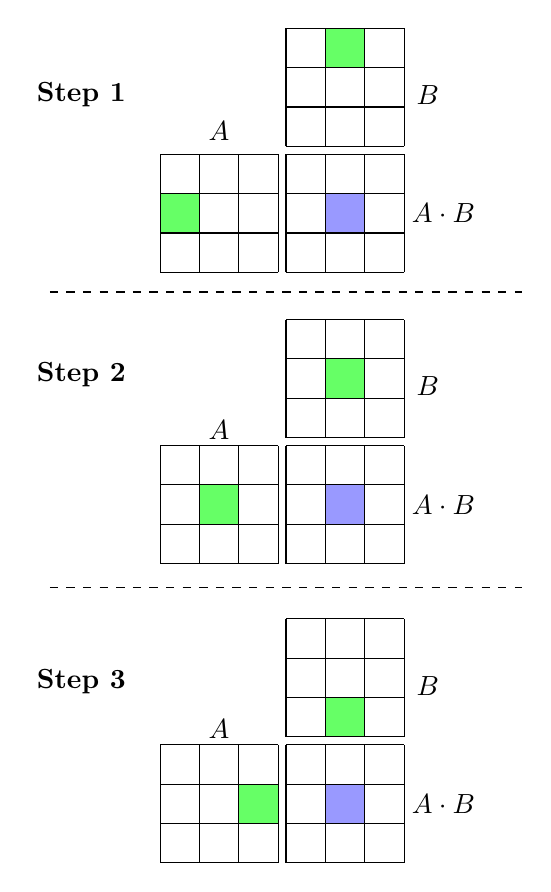
\begin{tikzpicture}
	\node at (-0.85,1.8) {$A$};
	\node at (1.8,2.25) {$B$};
	\node at (2.0,0.75) {$A \cdot B$};
	\node at (0.75,0.75) [rectangle,fill=blue!40,minimum width=0.5cm, minimum height=0.5cm] {};
	\node at (-1.35,0.75) [rectangle,fill=green!60,minimum width=0.5cm, minimum height=0.5cm] {};
	\node at (0.75,2.85) [rectangle,fill=green!60,minimum width=0.5cm, minimum height=0.5cm] {};
	\draw[step=0.5,black] grid (1.5,1.5);
	\draw[step=0.5,black,xshift=-1.6cm] grid (1.5,1.5);
	\draw[step=0.5,black,yshift=1.6cm] grid (1.5,1.5);
	\node at (-2.6,2.25) {\textbf{Step 1}};
	
	\draw[dashed] (-3.0,-0.25) to (3,-0.25);
	\draw[dashed] (-3.0,-4) to (3,-4);
		\node at (-0.85,-2) {$A$};
		\node at (1.8,-1.45) {$B$};
		\node at (2.0,-2.95) {$A \cdot B$};
		\node at (0.75,-2.95) [rectangle,fill=blue!40,minimum width=0.5cm, minimum height=0.5cm] {};
		\node at (-0.85,-2.95) [rectangle,fill=green!60,minimum width=0.5cm, minimum height=0.5cm] {};
		\node at (0.75,-1.35) [rectangle,fill=green!60,minimum width=0.5cm, minimum height=0.5cm] {};
		\draw[step=0.5,black,yshift=-3.7cm] grid (1.5,1.5);
		\draw[step=0.5,black,xshift=-1.6cm,yshift=-3.7cm] grid (1.5,1.5);
		\draw[step=0.5,black,yshift=-2.1cm] grid (1.5,1.5);
		\node at (-2.6,-1.3) {\textbf{Step 2}};
		
		\node at (-0.85,-5.8) {$A$};
		\node at (1.8,-5.25) {$B$};
		\node at (2.0,-6.75) {$A \cdot B$};
		\node at (0.75,-6.75) [rectangle,fill=blue!40,minimum width=0.5cm, minimum height=0.5cm] {};
		\node at (-0.35,-6.75) [rectangle,fill=green!60,minimum width=0.5cm, minimum height=0.5cm] {};
		\node at (0.75,-5.65) [rectangle,fill=green!60,minimum width=0.5cm, minimum height=0.5cm] {};
		\draw[step=0.5,black,yshift=-7.5cm] grid (1.5,1.5);
		\draw[step=0.5,black,xshift=-1.6cm,yshift=-7.5cm] grid (1.5,1.5);
		\draw[step=0.5,black,yshift=-5.9cm] grid (1.5,1.5);
		\node at (-2.6,-5.2) {\textbf{Step 3}};
		
\end{tikzpicture}
\centering
\label{fig:multiply}
\caption{Multiplication of $A$ and $B$ using shared memory}
\end{figure}

\subsection*{Checking if a matrix is the identity matrix}
We need a procedure which checks if a given matrix $A$ of dimension $n$-by-$n$ is equal to the identity matrix $I_n$. Formally defined:
\begin{equation*}
is\_id(A) := \begin{cases}
1 & \text{if } A \text{ has 1's in the diagonal, and 0's elsewhere}\\
0 & \text{otherwise}
\end{cases}
\end{equation*}
So $is\_id$ maps a matrix of $\mathbb{R}^{n \times n}$ to a single value $\{0,1 \}$. Therefore a implementation of $is\_id$ can be done efficiently using a \textbf{reduction}.  \\
We adapted the code from the CUDA 7.5 samples directory, namely from \texttt{/samples/6\_Advanced/reduction/}. The sample code is based on the whitepaper from Harris \cite{Harris2010} and optimizes the reduction for a summation of an array. The modification we did was that instead of summing up all array entries we used a auxiliary function $f_{acc}$ which takes an entry and its index as input and is returns 1 if  the value and the index to not match with the definition of the identity matrix. Formally:
\begin{equation}
f_{acc}(A_{i,j}) := \begin{cases} 1 & \text{if }i = j \text{ and } |A_{i,j}-1| \geq \varepsilon\\
1 & \text{if } i \neq j \text{ and } |A_{i,j}| \geq \varepsilon\\
0 & \text{otherwise}	\end{cases}
\end{equation}
Note that due to the limited floating point representation, a rounding error variable $\varepsilon$ must be chosen that should be close to 0, e.g. $\varepsilon = 10^{-6}$. \\
Our modified reduction computes $\sum_{i=0,j=0}^{n,n} f_{acc}(A_{i,j})$, so if the matrix $A$ matches the definition of the identity matrix the sum will be 0, if at least one entry of the matrix does not match the definition of the identity matrix, then the sum will be greater than 0.

\subsection*{LU decomposition}
To store the L and the U matrix, only one array of size $n^2$ is needed, because of the fixed 0s and 1s. For example the matrices
\begin{equation*}
 L = \begin{pmatrix} l_{11}  & 0 & 0\\ 
l_{21} & l_{22} & 0\\
l_{31} & l_{32} & l_{33}
\end{pmatrix}, U = \begin{pmatrix} 1 & u_{12} & u_{13}\\
0 & 1 & u_{23}\\
0 & 0 & 1\\
\end{pmatrix} 
\end{equation*}
Can be stored as
\begin{equation*}
LU = \begin{pmatrix} l_{11}  &  u_{12} & u_{13}\\
l_{21} & l_{22} & u_{23}\\
l_{31} & l_{32} & l_{33}
\end{pmatrix}
\end{equation*}
and thereby reducing the memory requirements by half.
\vspace{0.3cm}\\
The computation of the LU matrices and the row-permutation is separated into the following steps:
\begin{enumerate}
	\item Find Pivot, i.e. find row with the maximal absolute value in first column.\\
	This can be done efficiently on the GPU using a \textbf{reduction}. Like with the check for identity matrix we used the sample reduction in \texttt{/samples/6\_Advanced/reduction/} by Harris \cite{Harris2010}.
	\item Divide the pivot-row by pivot. Because the single computations do not depend on each other one grid equal to the side of the row can be launched. Each thread of the grid divides exactly one element of the row by the pivot. 
	\item Swap rows. This is application the row-permutation. Like before, each thread will swap exactly one item of the pivot row with the item in the first row.
	\item Update sub-matrix. As mentioned in section (\ref{sec:problem}) each element in the (n-1)-by-(n-1) sub-matrix needs to be subtracted by the product of the corresponding elements in the first row and first column. Every entry of this sub-matrix is updated by one thread. So the grid launched to do this task if of size (n-1)-by-(n-1)
	\item Process sub-matrix (recursive step)
\end{enumerate}
The last step would involve a recursive call to the procedure to itself. For performance reasons, the recursive algorithm was transformed into an iterative algorithm.
\subsection*{Matrix inversion of LU matrix}
As stated in section (\ref{sec:problem}), each column of the inverse matrix is computed separately by solving a linear equation. Because each linear equation is independent from the others, they can be solved in parallel. So a grid of size $n$ is launched, where each thread solves exactly one linear equation.  
